\documentclass{standalone}
\usepackage{tikz}
\usetikzlibrary{patterns}
\usetikzlibrary{positioning}
\usetikzlibrary{patterns, positioning}
\usetikzlibrary{shapes.misc}
\usepackage[outline]{contour}
\contourlength{1.5pt} 


\begin{document}
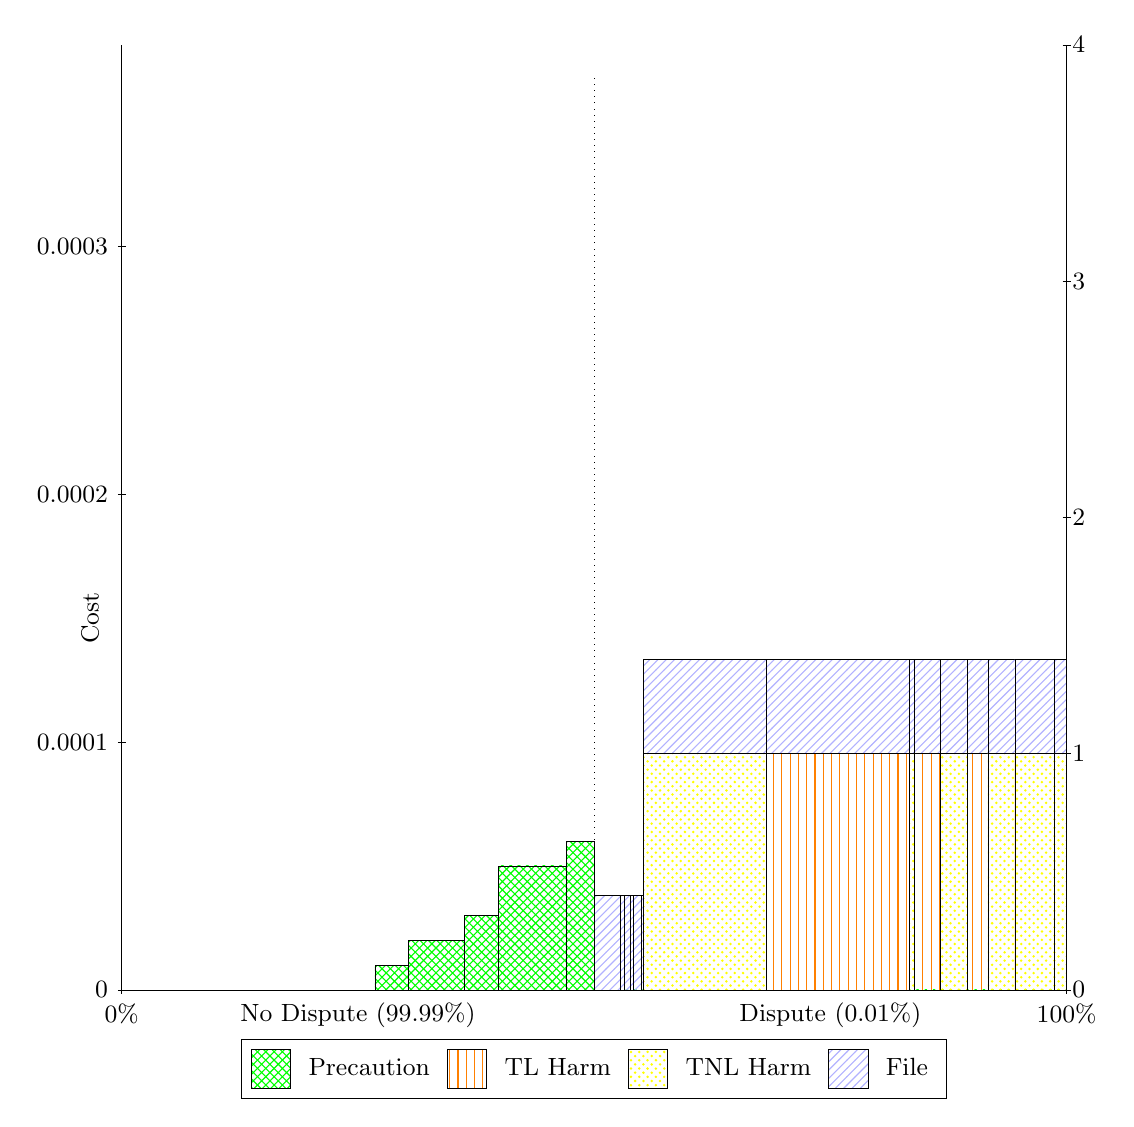
\begin{tikzpicture}
\draw[pattern=crosshatch, pattern color=green,draw=black,very thin] (4.7156,2.5) rectangle (5.1452,2.8147);
\draw[pattern=crosshatch, pattern color=green,draw=black,very thin] (5.1452,2.5) rectangle (5.8547,3.1293);
\draw[pattern=crosshatch, pattern color=green,draw=black,very thin] (5.8547,2.5) rectangle (6.2843,3.444);
\draw[pattern=crosshatch, pattern color=green,draw=black,very thin] (6.2843,2.5) rectangle (7.1452,4.0733);
\draw[pattern=crosshatch, pattern color=green,draw=black,very thin] (7.1452,2.5) rectangle (7.5,4.388);
\draw[pattern=north east lines, pattern color=blue!30,draw=black,very thin] (7.5,2.5) rectangle (7.8373,3.7);
\draw[pattern=crosshatch, pattern color=green,draw=black,very thin] (7.8373,2.5) rectangle (7.8823,2.5);
\draw[pattern=north east lines, pattern color=blue!30,draw=black,very thin] (7.8373,2.5) rectangle (7.8823,3.7);
\draw[pattern=crosshatch, pattern color=green,draw=black,very thin] (7.8823,2.5) rectangle (7.9568,2.5001);
\draw[pattern=north east lines, pattern color=blue!30,draw=black,very thin] (7.8823,2.5001) rectangle (7.9568,3.7001);
\draw[pattern=crosshatch, pattern color=green,draw=black,very thin] (7.9568,2.5) rectangle (8.0018,2.5001);
\draw[pattern=north east lines, pattern color=blue!30,draw=black,very thin] (7.9568,2.5001) rectangle (8.0018,3.7001);
\draw[pattern=crosshatch, pattern color=green,draw=black,very thin] (8.0018,2.5) rectangle (8.0921,2.5002);
\draw[pattern=north east lines, pattern color=blue!30,draw=black,very thin] (8.0018,2.5002) rectangle (8.0921,3.7002);
\draw[pattern=crosshatch, pattern color=green,draw=black,very thin] (8.0921,2.5) rectangle (8.1293,2.5002);
\draw[pattern=north east lines, pattern color=blue!30,draw=black,very thin] (8.0921,2.5002) rectangle (8.1293,3.7002);
\draw[pattern=crosshatch dots, pattern color=yellow,draw=black,very thin] (8.1293,2.5) rectangle (9.6897,5.5);
\draw[pattern=north east lines, pattern color=blue!30,draw=black,very thin] (8.1293,5.5) rectangle (9.6897,6.7);
\draw[pattern=vertical lines, pattern color=orange,draw=black,very thin] (9.6897,2.5) rectangle (11.502,5.5);
\draw[pattern=north east lines, pattern color=blue!30,draw=black,very thin] (9.6897,5.5) rectangle (11.502,6.7);
\draw[pattern=crosshatch, pattern color=green,draw=black,very thin] (11.502,2.5) rectangle (11.564,2.5);
\draw[pattern=crosshatch dots, pattern color=yellow,draw=black,very thin] (11.502,2.5) rectangle (11.564,5.5);
\draw[pattern=north east lines, pattern color=blue!30,draw=black,very thin] (11.502,5.5) rectangle (11.564,6.7);
\draw[pattern=crosshatch, pattern color=green,draw=black,very thin] (11.564,2.5) rectangle (11.899,2.5);
\draw[pattern=vertical lines, pattern color=orange,draw=black,very thin] (11.564,2.5) rectangle (11.899,5.5);
\draw[pattern=north east lines, pattern color=blue!30,draw=black,very thin] (11.564,5.5) rectangle (11.899,6.7);
\draw[pattern=crosshatch, pattern color=green,draw=black,very thin] (11.899,2.5) rectangle (12.244,2.5001);
\draw[pattern=crosshatch dots, pattern color=yellow,draw=black,very thin] (11.899,2.5001) rectangle (12.244,5.5001);
\draw[pattern=north east lines, pattern color=blue!30,draw=black,very thin] (11.899,5.5001) rectangle (12.244,6.7001);
\draw[pattern=crosshatch, pattern color=green,draw=black,very thin] (12.244,2.5) rectangle (12.5,2.5001);
\draw[pattern=vertical lines, pattern color=orange,draw=black,very thin] (12.244,2.5001) rectangle (12.5,5.5001);
\draw[pattern=north east lines, pattern color=blue!30,draw=black,very thin] (12.244,5.5001) rectangle (12.5,6.7001);
\draw[pattern=crosshatch, pattern color=green,draw=black,very thin] (12.5,2.5) rectangle (12.843,2.5001);
\draw[pattern=crosshatch dots, pattern color=yellow,draw=black,very thin] (12.5,2.5001) rectangle (12.843,5.5001);
\draw[pattern=north east lines, pattern color=blue!30,draw=black,very thin] (12.5,5.5001) rectangle (12.843,6.7001);
\draw[pattern=crosshatch, pattern color=green,draw=black,very thin] (12.843,2.5) rectangle (12.848,2.5001);
\draw[pattern=vertical lines, pattern color=orange,draw=black,very thin] (12.843,2.5001) rectangle (12.848,5.5001);
\draw[pattern=north east lines, pattern color=blue!30,draw=black,very thin] (12.843,5.5001) rectangle (12.848,6.7001);
\draw[pattern=crosshatch, pattern color=green,draw=black,very thin] (12.848,2.5) rectangle (13.349,2.5002);
\draw[pattern=crosshatch dots, pattern color=yellow,draw=black,very thin] (12.848,2.5002) rectangle (13.349,5.5002);
\draw[pattern=north east lines, pattern color=blue!30,draw=black,very thin] (12.848,5.5002) rectangle (13.349,6.7002);
\draw[pattern=crosshatch, pattern color=green,draw=black,very thin] (13.349,2.5) rectangle (13.5,2.5002);
\draw[pattern=crosshatch dots, pattern color=yellow,draw=black,very thin] (13.349,2.5002) rectangle (13.5,5.5002);
\draw[pattern=north east lines, pattern color=blue!30,draw=black,very thin] (13.349,5.5002) rectangle (13.5,6.7002);
\draw[black,very thin] (1.5,2.5) -- (1.5,14.5);
\node[font=\small,rotate=90,text=black, anchor=center] at (1.1, 7.2199) {Cost};
\draw[black,very thin] (1.45,2.5) -- (1.55,2.5);
\node[font=\small,text=black, anchor=east] at (1.45, 2.5) {0};
\draw[black,very thin] (1.45,5.6466) -- (1.55,5.6466);
\node[font=\small,text=black, anchor=east] at (1.45, 5.6466) {0.0001};
\draw[black,very thin] (1.45,8.7933) -- (1.55,8.7933);
\node[font=\small,text=black, anchor=east] at (1.45, 8.7933) {0.0002};
\draw[black,very thin] (1.45,11.94) -- (1.55,11.94);
\node[font=\small,text=black, anchor=east] at (1.45, 11.94) {0.0003};

\draw[black,dotted,very thin] (7.5,2.86) -- (7.5,14.14);
\draw[black,very thin] (13.5,2.5) -- (13.5,14.5);
\draw[black,very thin] (13.45,2.5) -- (13.55,2.5);
\node[font=\small,text=black, anchor=west] at (13.45, 2.5) {0};
\draw[black,very thin] (13.45,5.5) -- (13.55,5.5);
\node[font=\small,text=black, anchor=west] at (13.45, 5.5) {1};
\draw[black,very thin] (13.45,8.5) -- (13.55,8.5);
\node[font=\small,text=black, anchor=west] at (13.45, 8.5) {2};
\draw[black,very thin] (13.45,11.5) -- (13.55,11.5);
\node[font=\small,text=black, anchor=west] at (13.45, 11.5) {3};
\draw[black,very thin] (13.45,14.5) -- (13.55,14.5);
\node[font=\small,text=black, anchor=west] at (13.45, 14.5) {4};

\draw[black,very thin] (1.5,2.5) -- (13.5,2.5);
\draw[black,very thin] (1.5,2.45) -- (1.5,2.55);
\node[font=\small,text=black, anchor=north] at (1.5, 2.45) {0\%};
\draw[black,very thin] (13.5,2.45) -- (13.5,2.55);
\node[font=\small,text=black, anchor=north] at (13.5, 2.45) {100\%};

\node[font=\small,text=black,anchor=south] at (4.5, 1.9) {No\ Dispute\ (99.99\%)};
\node[font=\small,text=black,anchor=south] at (10.5, 1.9) {Dispute\ (0.01\%)};
\draw (7.5,2.5) node (B) {};
\begin{scope}[align=center]
\matrix[scale=0.5,draw=black,below=0.5cm of B,nodes={draw},column sep=0.1cm]{
\node[rectangle,draw,minimum width=0.5cm,minimum height=0.5cm,pattern=crosshatch, pattern color=green]{}; & \node[draw=none,font=\small,text=black]{Precaution}; &
\node[rectangle,draw,minimum width=0.5cm,minimum height=0.5cm,pattern=vertical lines, pattern color=orange]{}; & \node[draw=none,font=\small,text=black]{TL Harm}; &
\node[rectangle,draw,minimum width=0.5cm,minimum height=0.5cm,pattern=crosshatch dots, pattern color=yellow]{}; & \node[draw=none,font=\small,text=black]{TNL Harm}; &
\node[rectangle,draw,minimum width=0.5cm,minimum height=0.5cm,pattern=north east lines, pattern color=blue!30]{}; & \node[draw=none,font=\small,text=black]{File}; \\\\
};\end{scope}

\end{tikzpicture}
\end{document}